% -----------------------------*- LaTeX -*------------------------------
\documentclass[UTF8]{report}
% ------------------------------------------------------------------------
% Packages
% ------------------------------------------------------------------------
\usepackage{ctex} % 支持中文
\usepackage[body={7in, 9in},left=1in,right=1in]{geometry} % 改变页边距
\usepackage{amsmath} % AMS 的数学宏包
\usepackage{amsfonts} % AMS 的数学字体宏包
\usepackage{amssymb} % AMS 符号库
\usepackage{bm} % 数学公式中的黑斜体
\usepackage{amsthm} % AMS 的定理环境宏包
\usepackage{graphicx} % 插图
\usepackage{subfigure} % 插子图
\usepackage{nicefrac} % 好看的分数
\usepackage{mathrsfs} % mathscr font
\usepackage{caption} % caption
\usepackage{algorithm,algorithmicx} % 伪代码支持宏包
\usepackage[noend]{algpseudocode} % 伪代码
\usepackage{fancyhdr} % 设置页眉、页脚
\usepackage{adjustbox} % 图片尺寸自动调整
\usepackage{esint} % 积分符号
\usepackage{mathtools} % 数学宏包的重要补充
\usepackage{upgreek} % 数学环境的直立希腊字母
\usepackage{enumitem} % 使用enumitem宏包, 改变列表项的格式
\usepackage{color} % 支持彩色
\usepackage{extarrows} % 任意长度的箭头
\usepackage{tikz} % 绘图
\usepackage{forest} % 绘树
\usepackage{xcolor} % 颜色宏包
\usepackage{breqn} % 公式自动换行
\usepackage{fontsize} % 字体大小
\usepackage[framemethod=TikZ]{mdframed} % 给文字加框
\usepackage{fontspec} % 字体库
\usepackage{bigstrut} % 用于表格中的换行
\usepackage{multirow} % 表格中多行单元格合并
\usepackage{multicol} % 表格中多列单元格合并
\usepackage{longtable} % 长表格
\usepackage{rotating} % 旋转图形和表格      以上三者用于绘制三线表
\usepackage{booktabs} % 三线表宏包
\usepackage{scribe} % Scribe 模板
\usepackage{diagbox} % 表格斜线
\usepackage{listings} % 插入代码
\usepackage{verbatim} % 多行注释
\usepackage{ifplatform} % 检测编译平台
\usepackage{hyperref} % 超链接
\usepackage{pifont} % 圆圈数字
\usetikzlibrary{shapes.geometric, arrows} % 引入流程图需要的库
\usetikzlibrary{automata} % 引入automata库
\usetikzlibrary{shapes,arrows,positioning,chains} % 引入positioning库
% ------------------------------------------------------------------------
% Macros
% ------------------------------------------------------------------------
%~~~~~~~~~~~~~~~
% Utility latin
%~~~~~~~~~~~~~~~
\newcommand{\ie}{\textit{i.e.}}
\newcommand{\eg}{\textit{e.g.}}
%~~~~~~~~~~~~~~~
% Environment shortcuts
%~~~~~~~~~~~~~~~
\newcommand{\balign}[1]{\ealign{\begin{align}#1\end{align}}}
\newcommand{\baligns}[1]{\ealigns{\begin{align*}#1\end{align*}}}
\newcommand{\bitemize}[1]{\eitemize{\begin{itemize}#1\end{itemize}}}
\newcommand{\benumerate}[1]{\eenumerate{\begin{enumerate}#1\end{enumerate}}}
%~~~~~~~~~~~~~~~
% Text with quads around it
%~~~~~~~~~~~~~~~
\newcommand{\qtext}[1]{\quad\text{#1}\quad}
%~~~~~~~~~~~~~~~
% Shorthand for math formatting
%~~~~~~~~~~~~~~~
\newcommand{\mbb}[1]{\mathbb{#1}}
\newcommand{\mbi}[1]{\boldsymbol{#1}} % Bold and italic (math bold italic)
\newcommand{\mbf}[1]{\mathbf{#1}}
\newcommand{\mc}[1]{\mathcal{#1}}
\newcommand{\mrm}[1]{\mathrm{#1}}
\newcommand{\tbf}[1]{\textbf{#1}}
\newcommand{\tsc}[1]{\textsc{#1}}
%\def\\langle {{\langle }}
%\def\\rangle {{\rangle }}
\newcommand{\sT}{\sf T}
\newcommand{\grad}{\nabla}
\newcommand{\Proj}{\Pi}
%~~~~~~~~~~~~~~~
% Common sets 定义数集符号
%~~~~~~~~~~~~~~~
\newcommand{\R}{\mathbb{R}}
\newcommand{\Z}{\mathbb{Z}}
\newcommand{\Q}{\mathbb{Q}}
\newcommand{\N}{\mathbb{N}}
\newcommand{\C}{\mathbb{C}}
\newcommand{\reals}{\mathbb{R}} % Real number symbol
\newcommand{\integers}{\mathbb{Z}} % Integer symbol
\newcommand{\rationals}{\mathbb{Q}} % Rational numbers
\newcommand{\naturals}{\mathbb{N}} % Natural numbers
\newcommand{\complex}{\mathbb{C}} % Complex numbers
%~~~~~~~~~~~~~~~
% Common functions
%~~~~~~~~~~~~~~~
\renewcommand{\exp}[1]{\operatorname{exp}\left(#1\right)} % Exponential
\newcommand{\indic}[1]{\mbb{I}\left(#1\right)} % Indicator function
\newcommand{\indicsub}[2]{\mbb{I}_{#2}\left(#1\right)} % Indicator function
\newcommand{\argmax}{\mathop\mathrm{arg\, max}} % Defining math symbols
\newcommand{\argmin}{\mathop\mathrm{arg\, min}}
\renewcommand{\arccos}{\mathop\mathrm{arccos}}
\newcommand{\dom}{\mathop\mathrm{dom}} % Domain
\newcommand{\range}{\mathop\mathrm{range}} % Range
\newcommand{\diag}{\mathop\mathrm{diag}}
\newcommand{\tr}{\mathop\mathrm{tr}}
\newcommand{\abs}{\mathop\mathrm{abs}}
\newcommand{\card}{\mathop\mathrm{card}}
\newcommand{\sign}{\mathop\mathrm{sign}}
\newcommand{\prox}{\mathrm{prox}} % prox
\newcommand{\rank}[1]{\mathrm{rank}(#1)}
\newcommand{\supp}[1]{\mathrm{supp}(#1)}
\newcommand{\norm}[1]{\lVert#1\rVert}
%~~~~~~~~~~~~~~~
% Common probability symbols
%~~~~~~~~~~~~~~~
\newcommand{\family}{\mathcal{P}} % probability family / statistical model
\newcommand{\iid}{\stackrel{\mathrm{iid}}{\sim}}
\newcommand{\ind}{\stackrel{\mathrm{ind}}{\sim}}
\newcommand{\E}{\mathbb{E}} % Expectation symbol
\newcommand{\Earg}[1]{\E\left[#1\right]}
\newcommand{\Esubarg}[2]{\E_{#1}\left[#2\right]}
\renewcommand{\P}{\mathbb{P}} % Probability symbol
\newcommand{\Parg}[1]{\P\left(#1\right)}
\newcommand{\Psubarg}[2]{\P_{#1}\left[#2\right]}
%\newcommand{\Cov}{\mrm{Cov}} % Covariance symbol
%\newcommand{\Covarg}[1]{\Cov\left[#1\right]}
%\newcommand{\Covsubarg}[2]{\Cov_{#1}\left[#2\right]}
%\newcommand{\model}{\mathcal{P}} % probability family / statistical model
%~~~~~~~~~~~~~~~
% Distributions
%~~~~~~~~~~~~~~~
%\newcommand{\Gsn}{\mathcal{N}}
%\newcommand{\Ber}{\textnormal{Ber}}
%\newcommand{\Bin}{\textnormal{Bin}}
%\newcommand{\Unif}{\textnormal{Unif}}
%\newcommand{\Mult}{\textnormal{Mult}}
%\newcommand{\NegMult}{\textnormal{NegMult}}
%\newcommand{\Dir}{\textnormal{Dir}}
%\newcommand{\Bet}{\textnormal{Beta}}
%\newcommand{\Gam}{\textnormal{Gamma}}
%\newcommand{\Poi}{\textnormal{Poi}}
%\newcommand{\HypGeo}{\textnormal{HypGeo}}
%\newcommand{\GEM}{\textnormal{GEM}}
%\newcommand{\BP}{\textnormal{BP}}
%\newcommand{\DP}{\textnormal{DP}}
%\newcommand{\BeP}{\textnormal{BeP}}
%\newcommand{\Exp}{\textnormal{Exp}}
%~~~~~~~~~~~~~~~
% Theorem-like environments
%~~~~~~~~~~~~~~~
%\theoremstyle{definition}
%\newtheorem{definition}{Definition}
%\newtheorem{example}{Example}
%\newtheorem{problem}{Problem}
%\newtheorem{lemma}{Lemma}
%~~~~~~~~~~~~~~~
% 组合数学的模板和作业里用到的一些宏包和自定义命令
%~~~~~~~~~~~~~~~
\renewcommand{\emph}[1]{\begin{kaishu}#1\end{kaishu}}
\newcommand{\falfac}[1]{^{\underline{#1}}}
\newcommand{\binomfrac}[2]{\frac{#1^{\underline{#2}}}{#2!}}
\newcommand{\ceil}[1]{\left\lceil #1 \right\rceil}
\newcommand{\floor}[1]{\left\lfloor #1 \right\rfloor}
\newcommand{\suminfty}[2]{\sum_{#1=#2}^{\infty}}
\newcommand{\suminftyk}[0]{\sum_{k=0}^{\infty}}
\newcommand{\sumint}[3]{\sum_{#1=#2}^{#3}}
\newcommand{\sumintk}[2]{\sum_{k=#1}^{#2}}
\newcommand{\suminti}[2]{\sum_{i=#1}^{#2}}
%~~~~~~~~~~~~~~~
% 定义新命令
%~~~~~~~~~~~~~~~
\newcommand*{\unit}[1]{\mathop{}\!\mathrm{#1}}
\newcommand*{\dif}{\mathop{}\!\mathrm{d}}%微分算子 d
\newcommand*{\pdif}{\mathop{}\!\partial}%偏微分算子
\newcommand*{\cdif}{\mathop{}\!\nabla}%协变导数、nabla 算子
\newcommand*{\laplace}{\mathop{}\!\Delta}%laplace 算子
\newcommand*{\deri}[1]{\mathrm{d} #1}
\newcommand*{\deriv}[2]{\frac{\mathrm{d} #1}{\mathrm{d} {#2}}}
\newcommand*{\derivh}[3]{\frac{\mathrm{d}^{#1} #2}{\mathrm{d} {#3^{#1}}}}
\newcommand*{\pderiv}[2]{\frac{\partial #1}{\partial {#2}}}
\newcommand*{\pderivh}[3]{\frac{\partial^{#1} #2}{\partial {#3^{#1}}}}
\newcommand*{\dderiv}[2]{\dfrac{\mathrm{d} #1}{\mathrm{d} {#2}}}
\newcommand*{\dderivh}[3]{\dfrac{\mathrm{d}^{#1} #2}{\mathrm{d} {#3^{#1}}}}
\newcommand*{\dpderiv}[2]{\dfrac{\partial #1}{\partial {#2}}}
\newcommand*{\dpderivh}[3]{\dfrac{\partial^{#1} #2}{\partial {#3^{#1}}}}
\newcommand{\me}[1]{\mathrm{e}^{#1}}%e 指数
\newcommand{\mi}{\mathrm{i}}%虚数单位
%\newcommand{\mc}{\mathrm{c}}%光速 定义与mathcal冲突
\newcommand{\red}[1]{\textcolor{red}{#1}}
\newcommand{\blue}[1]{\textcolor{blue}{#1}}
%\newcommand{\Rome}[1]{\setcounter{rome}{#1}\Roman{rome}}
%~~~~~~~~~~~~~~~
% 公式环境中箭头符号的简写
%~~~~~~~~~~~~~~~
\newcommand{\ra}{\rightarrow}
\newcommand{\Ra}{\Rightarrow}
\newcommand{\la}{\leftarrow}
\newcommand{\La}{\Leftarrow}
\newcommand{\lra}{\leftrightarrow}
\newcommand{\Lra}{\Leftrightarrow}
\newcommand{\lgla}{\longleftarrow}
\newcommand{\Lgla}{\Longleftarrow}
\newcommand{\lgra}{\longrightarrow}
\newcommand{\Lgra}{\Longrightarrow}
\newcommand{\lglra}{\longleftrightarrow}
\newcommand{\Lglra}{\Longleftrightarrow}
%~~~~~~~~~~~~~~~
% 一些数学的环境设置
%~~~~~~~~~~~~~~~
%\newcounter{counter_exm}\setcounter{counter_exm}{1}
%\newcounter{counter_prb}\setcounter{counter_prb}{1}
%\newcounter{counter_thm}\setcounter{counter_thm}{1}
%\newcounter{counter_lma}\setcounter{counter_lma}{1}
%\newcounter{counter_dft}\setcounter{counter_dft}{1}
%\newcounter{counter_clm}\setcounter{counter_clm}{1}
%\newcounter{counter_cly}\setcounter{counter_cly}{1}
\newtheorem{theorem}{{\hskip 1.7em \bf 定理}}
\newtheorem{lemma}[theorem]{\hskip 1.7em 引理}
\newtheorem{proposition}[theorem]{\hskip 1.7em 命题}
\newtheorem{claim}[theorem]{\hskip 1.7em 断言}
\newtheorem{corollary}[theorem]{\hskip 1.7em 推论}
% \newcommand{\problem}[1]{{\setlength{\parskip}{10pt}\noindent \bf{#1}}}
\newenvironment{solution}{{\noindent \bf 解 \quad}}{}
\newenvironment{remark}{{\noindent \bf 注 \quad}}{}
\newenvironment{definition}{{\noindent \bf 定义 \quad}}{}
\renewenvironment{proof}{{\setlength{\parskip}{7pt}\noindent\hskip 2em \bf 证明 \quad}}{\hfill$\qed$\par}
\newenvironment{example}{{\noindent\bf 例 \quad}}{\hfill$\qed$\par}
%\newenvironment{concept}[1]{{\bf #1\quad} \begin{kaishu}} {\end{kaishu}\par}
%~~~~~~~~~~~~~~~
% 本.tex文档中特殊定义命令
%~~~~~~~~~~~~~~~
\newcommand{\lno}[1]{\overline{#1}}
\newcommand{\NP}{\mathrm{NP}}
\newcommand{\coNP}{\mathrm{coNP}}
% \newcommand{\ISO}{\mathrm{ISO}}
\newcommand{\SAT}{\mathrm{SAT}}
\newcommand{\USAT}{\mathrm{USAT}}
% \newcommand{\threeSAT}{\mathrm{3\text{-}SAT}}
\renewcommand{\P}{\mathrm{P}}
% \mathchardef\mhyphen="2D
% \newcommand{\CNF}{\mathrm{CNF}}
% \newcommand{\DNF}{\mathrm{DNF}}
% \newcommand{\SetSp}{\mathrm{SET\text{-}SPLITTING}}
% \newcommand{\PUZZLE}{\mathrm{PUZZLE}}
% \newcommand{\SPATH}{\mathrm{SPATH}}
% \newcommand{\LPATH}{\mathrm{LPATH}}
% \newcommand{\UHAMPATH}{\mathrm{UHAMPATH}}
\newcommand{\SPACE}{\mathrm{SPACE}}
\newcommand{\NSPACE}{\mathrm{NSPACE}}
\newcommand{\PSPACE}{\mathrm{PSPACE}}
\newcommand{\NPSPACE}{\mathrm{NPSPACE}}
\newcommand{\DFA}{\mathrm{DFA}}
\newcommand{\NFA}{\mathrm{NFA}}
\newcommand{\TQBF}{\mathrm{TQBF}}
% \newcommand{\L}{\mathrm{L}}
\renewcommand{\O}{\mathrm{O}}
\newcommand{\NL}{\mathrm{NL}}
\newcommand{\coNL}{\mathrm{coNL}}
\newcommand{\LADDER}{\mathrm{LADDER_{DFA}}}
\newcommand{\hd}{\mathrm{\text{-}hard}}
\newcommand{\ADD}{\mathrm{ADD}}
\newcommand{\STCN}{\mathrm{STRONGLY\text{-}CONNECTED}}
\newcommand{\PATH}{\mathrm{PATH}}
\newcommand{\A}{\mathrm{A}}
%使用align环境公式换页
\allowdisplaybreaks[4]

\definecolor{dkgreen}{rgb}{0,0.6,0}
\definecolor{gray}{rgb}{0.5,0.5,0.5}
\definecolor{mauve}{rgb}{0.58,0,0.82}
\lstset{
  frame=tb,
  aboveskip=3mm,
  belowskip=3mm,
  showstringspaces=false,
  columns=flexible,
  framerule=1pt,
  rulecolor=\color{gray!35},
  backgroundcolor=\color{gray!5},
  basicstyle={\small\ttfamily},
  numbers=none,
  numberstyle=\tiny\color{gray},
  keywordstyle=\color{blue},
  commentstyle=\color{dkgreen},
  stringstyle=\color{mauve},
  breaklines=true,
  breakatwhitespace=true,
  tabsize=3,
}

\hypersetup{
    colorlinks=true,
    linkcolor=blue,
    filecolor=magenta,      
    urlcolor=cyan,
    citecolor=green,
}

\urlstyle{same}

\tikzstyle{startstop} = [rectangle, rounded corners, minimum width=3cm, minimum height=1cm,text centered, draw=black, fill=red!30]
\tikzstyle{process} = [rectangle, minimum width=3cm, minimum height=1cm, text centered, draw=black, fill=orange!30]
\tikzstyle{decision} = [diamond, minimum width=3cm, minimum height=1cm, text centered, draw=black, fill=green!30]
\tikzstyle{arrow} = [thick,->,>=stealth]



\ifwindows
    \setmainfont{Times New Roman}
    \setsansfont{Times New Roman}
    \setmonofont{Consolas}
    \setCJKmainfont{SimHei}
    \setCJKsansfont{SimSun}
    \setCJKmonofont{FangSong}
\fi

\ifmacosx
    \setmainfont{Times New Roman}
    \setsansfont{Times New Roman}
    \setmonofont{Menlo}
    \setCJKmainfont{Heiti SC}
    \setCJKsansfont{STSong}
    \setCJKmonofont{STFangsong}
\fi

\punctstyle{kaiming}

\begin{document}

\pagestyle{fancy}

\reporttype{Report}                 % required
\course{Lab of Computer Network} 				% optional
\coursetitle{TCP-Stack-2}	    % optional
\semester{Fall 2024}			    % optional
\lecturer{Wu Qinghua}			% optional
\scribe{2022K8009929010 Zhang Jiawei}			% required
\lecturenumber{14}				% required (must be a number)
\lecturedate{December 16}			% required (omit year)
\maketitle

\section{实验内容}

\begin{enumerate}

    \item \textbf{丢包恢复}
    \begin{itemize}
        \item 执行 \texttt{create\_randfile.sh},生成待传输数据文件 \texttt{client-input.dat}。
        \item 运行给定网络拓扑 (\texttt{tcp\_topo\_loss.py})。
        \item 在节点 \texttt{h1} 上执行 TCP 程序:
        \begin{itemize}
            \item 执行脚本 (\texttt{disable\_offloading.sh} 和 \texttt{disable\_tcp\_rst.sh}),禁止协议栈的相应功能。
            \item 在 \texttt{h1} 上运行 TCP 协议栈的服务器模式:
            \texttt{./tcp\_stack server 10001}。
        \end{itemize}
        \item 在节点 \texttt{h2} 上执行 TCP 程序:
        \begin{itemize}
            \item 执行脚本 (\texttt{disable\_offloading.sh} 和 \texttt{disable\_tcp\_rst.sh}),禁止协议栈的相应功能。
            \item 在 \texttt{h2} 上运行 TCP 协议栈的客户端模式:
            \texttt{./tcp\_stack client 10.0.0.1 10001}。
        \end{itemize}
        \item \texttt{Client} 发送文件 \texttt{client-input.dat} 给 \texttt{server},\texttt{server} 将收到的数据存储到文件 \texttt{server-output.dat}。
        \item 使用 \texttt{md5sum} 比较两个文件是否完全相同。
        \item 使用 \texttt{tcp\_stack.py} 替换两端任意一方,对端都能正确处理数据收发。
    \end{itemize}

    \item \textbf{拥塞控制}
    \begin{itemize}
        \item 执行 \texttt{create\_randfile.sh},生成待传输数据文件 \texttt{client-input.dat}。
        \item 运行给定网络拓扑 (\texttt{tcp\_topo\_loss.py})。
        \item 在节点 \texttt{h1} 上执行 TCP 程序:
        \begin{itemize}
            \item 执行脚本 (\texttt{disable\_offloading.sh} 和 \texttt{disable\_tcp\_rst.sh}),禁止协议栈的相应功能。
            \item 在 \texttt{h1} 上运行 TCP 协议栈的服务器模式:
            \texttt{./tcp\_stack server 10001}。
        \end{itemize}
        \item 在节点 \texttt{h2} 上执行 TCP 程序:
        \begin{itemize}
            \item 执行脚本 (\texttt{disable\_offloading.sh} 和 \texttt{disable\_tcp\_rst.sh}),禁止协议栈的相应功能。
            \item 在 \texttt{h2} 上运行 TCP 协议栈的客户端模式:
            \texttt{./tcp\_stack client 10.0.0.1 10001}。
        \end{itemize}
        \item \texttt{Client} 发送文件 \texttt{client-input.dat} 给 \texttt{server},\texttt{server} 将收到的数据存储到文件\texttt{server-output.dat}。
        \item 使用 \texttt{md5sum} 比较两个文件是否完全相同。
        \item 记录 \texttt{h2} 中每次 \texttt{cwnd} 调整的时间和相应值,呈现到二维坐标图中。
    \end{itemize}

\end{enumerate}

\section{实验过程}

\subsection{丢包恢复}

\begin{enumerate}
    \item \tbf{重传定时器操作}
    
    本次实验中,我们需要实现定时器的设置、更新、关闭、扫描操作。
    
    设置操作较为简单,先检查是否有定时器,如果没有则直接设置定时器类型为重传定时器,启用并设置超时时间,设置重传次数为0;如果已有定时器,则更新超时时间。最后把定时器加入定时器链表。

    更新操作也较为简单,若已建立的连接发送队列为空,则关闭并删除定时器,唤醒发送数据进程。

    关闭操作也较为简单,与更新操作类似,只是判断条件改为定时器队列不为空。

    扫描操作则需要遍历定时器链表,减少每个定时器的剩余时间,若剩余时间小于等于0,即超时,则进行处理:重传次数未达上限则重传数据包,重传次数达到上限则直接断开连接,释放资源。扫描操作通过一个线程每10秒进行一次扫描。

    代码如下:

    \begin{lstlisting}[language=C]
        // set the restrans timer of a tcp sock, by adding the timer into timer_list
        void tcp_set_retrans_timer(struct tcp_sock *tsk)
        {
            if (tsk->retrans_timer.enable) {
                tsk->retrans_timer.timeout = TCP_RETRANS_INTERVAL_INITIAL;
                return;
            }
            tsk->retrans_timer.type = TIMER_TYPE_RETRANS;
            tsk->retrans_timer.enable = 1;
            tsk->retrans_timer.timeout = TCP_RETRANS_INTERVAL_INITIAL;
            tsk->retrans_timer.retrans_time = 0;
        
            pthread_mutex_lock(&retrans_timer_list_lock);
            list_add_tail(&tsk->retrans_timer.list, &retrans_timer_list);
            pthread_mutex_unlock(&retrans_timer_list_lock);
        }
        
        void tcp_update_retrans_timer(struct tcp_sock *tsk)
        {
            if (list_empty(&tsk->send_buf) && tsk->retrans_timer.enable) {
                tsk->retrans_timer.enable = 0;
                list_delete_entry(&tsk->retrans_timer.list);
                wake_up(tsk->wait_send);
            }
        }
        
        void tcp_unset_retrans_timer(struct tcp_sock *tsk)
        {
            if (!list_empty(&tsk->retrans_timer.list)) {
                tsk->retrans_timer.enable = 0;
                list_delete_entry(&tsk->retrans_timer.list);
                wake_up(tsk->wait_send);
            }
            else
                log(ERROR, "unset an empty retrans timer\n");
        }
        
        void tcp_scan_retrans_timer_list(void)
        {
            struct tcp_sock *tsk;
            struct tcp_timer *time_entry, *time_q;
        
            pthread_mutex_lock(&retrans_timer_list_lock);
            
            list_for_each_entry_safe(time_entry, time_q, &retrans_timer_list, list) {
                time_entry->timeout -= TCP_RETRANS_SCAN_INTERVAL;
                tsk = retranstimer_to_tcp_sock(time_entry);
                if (time_entry->timeout <= 0) {
                    if(time_entry->retrans_time >= MAX_RETRANS_NUM && tsk->state != TCP_CLOSED){
                        list_delete_entry(&time_entry->list);
                        if (!tsk->parent)
                            tcp_unhash(tsk);
                            
                        wait_exit(tsk->wait_connect);
                        wait_exit(tsk->wait_accept);
                        wait_exit(tsk->wait_recv);
                        wait_exit(tsk->wait_send);
                        
                        tcp_set_state(tsk, TCP_CLOSED);
                        tcp_send_control_packet(tsk, TCP_RST);
                    }
                    else if (tsk->state != TCP_CLOSED) {
                        time_entry->retrans_time += 1;
                        log(DEBUG, "retrans time: %d\n", time_entry->retrans_time);
                        time_entry->timeout = TCP_RETRANS_INTERVAL_INITIAL;
                        tcp_retrans_send_buffer(tsk);
                    }
                }
            }
        
            pthread_mutex_unlock(&retrans_timer_list_lock);
        }
        
        void *tcp_retrans_timer_thread(void *arg)
        {
            init_list_head(&retrans_timer_list);
            while(1){
                usleep(TCP_RETRANS_SCAN_INTERVAL);
                tcp_scan_retrans_timer_list();
            }
        
            return NULL;
        }
    \end{lstlisting}

    \item \tbf{发送队列}
    
    对于发送队列,我们需要实现数据包的添加、更新、重传操作,都比较简单。

    添加操作只需将数据包加入发送队列即可。注意这里需要使用互斥锁保护发送队列。

    更新操作是指遍历队列,将队列中序列号小于收到的 ACK 的数据包删除。这里同样需要使用互斥锁保护发送队列。

    重传操作是指超时未收到 ACK 时,将队列中第一个的数据包重传。我将队列中第一个数据包的TCP序列号、确认号等信息更新之后,再计算出数据长度和发送窗口大小,将数据包发送出去。

    代码如下:

    \begin{lstlisting}[language=C]
        // Add a packet to the TCP send buffer
        void tcp_send_buffer_add_packet(struct tcp_sock *tsk, char *packet, int len) {
            send_buffer_entry_t *send_buffer_entry = (send_buffer_entry_t *)malloc(sizeof(send_buffer_entry_t));
            memset(send_buffer_entry, 0, sizeof(send_buffer_entry_t));
        
            send_buffer_entry->packet = (char *)malloc(len);
            send_buffer_entry->len = len;
            memcpy(send_buffer_entry->packet, packet, len);
        
            init_list_head(&send_buffer_entry->list);
        
            list_add_tail(&send_buffer_entry->list, &tsk->send_buf);
        }
        
        //Update the TCP send buffer based on the acknowledgment number
        void tcp_update_send_buffer(struct tcp_sock *tsk, u32 ack) {
            send_buffer_entry_t *send_buffer_entry, *send_buffer_entry_q;
        
            list_for_each_entry_safe(send_buffer_entry, send_buffer_entry_q, &tsk->send_buf, list) {
                struct tcphdr *tcp = packet_to_tcp_hdr(send_buffer_entry->packet);
                u32 seq = ntohl(tcp->seq);
        
                // If the sequence number is less than the acknowledgment number, delete the entry
                if (less_than_32b(seq, ack)) {
                    list_delete_entry(&send_buffer_entry->list);
                    free(send_buffer_entry->packet);
                    free(send_buffer_entry);
                }
            }
        }
        
        // Retransmit the first packet in the TCP send buffer when ack time exceed
        int tcp_retrans_send_buffer(struct tcp_sock *tsk) {
            if (list_empty(&tsk->send_buf)) {
                log(ERROR, "no packet to retrans\n");
                pthread_mutex_unlock(&tsk->send_buf_lock);
                return 0;
            }
        
            // Retrieve the first send buffer entry
            send_buffer_entry_t *first_send_buffer_entry = list_entry(tsk->send_buf.next, send_buffer_entry_t, list);
        
            char *packet = (char *)malloc(first_send_buffer_entry->len);
        
            // Copy the packet data and update TCP sequence and acknowledgment numbers
            memcpy(packet, first_send_buffer_entry->packet, first_send_buffer_entry->len);
            struct iphdr *ip = packet_to_ip_hdr(packet);
            struct tcphdr *tcp = packet_to_tcp_hdr(packet);
            tcp->ack = htonl(tsk->rcv_nxt);
            tcp->checksum = tcp_checksum(ip, tcp);
            ip->checksum = ip_checksum(ip);
        
            // Calculate TCP data length and update TCP send window
            int tcp_data_len = ntohs(ip->tot_len) - IP_BASE_HDR_SIZE - TCP_BASE_HDR_SIZE;
            tsk->snd_wnd -= tcp_data_len;
        
            log(DEBUG, "retrans seq: %u\n", ntohl(tcp->seq));
        
            // Send the packet
            ip_send_packet(packet, first_send_buffer_entry->len);
            return 1;
        }
    \end{lstlisting}
    
    \item \tbf{接收队列}
    
    对于接收队列,我们需要实现数据包的添加、移动操作,稍微繁琐。

    添加操作要将接收到的数据包按照 seq 顺序插入接收队列中,若出现重复数据包则直接丢弃,然后将有效的数据包插入队列中。

    移动操作首先遍历接收队列,找到与当前 \texttt{rcv\_nxt} 匹配的数据包,然后写入环形缓冲区,唤醒接收进程,更新 \texttt{rcv\_nxt}。注意环形缓冲区需要使用互斥锁保护。

    代码如下:

    \begin{lstlisting}[language=C]
        // Add an packet to the TCP receive buffer
        int tcp_recv_ofo_buffer_add_packet(struct tcp_sock *tsk, struct tcp_cb *cb) {
            if (cb->pl_len <= 0)
                return 0;
            recv_ofo_buf_entry_t *recv_ofo_entry = (recv_ofo_buf_entry_t *)malloc(sizeof(recv_ofo_buf_entry_t));
            recv_ofo_entry->seq = cb->seq;
            recv_ofo_entry->seq_end = cb->seq_end;
            recv_ofo_entry->len = cb->pl_len;
            recv_ofo_entry->data = (char *)malloc(cb->pl_len);
            memcpy(recv_ofo_entry->data, cb->payload, cb->pl_len);
        
            init_list_head(&recv_ofo_entry->list);
            // insert the new entry at the correct position
            recv_ofo_buf_entry_t *entry, *entry_q;
            list_for_each_entry_safe (entry, entry_q, &tsk->rcv_ofo_buf, list) {
                if (recv_ofo_entry->seq == entry->seq)
                    return 1; // same seq, do not add
                if (less_than_32b(recv_ofo_entry->seq, entry->seq)) {
                    list_add_tail(&recv_ofo_entry->list, &entry->list);
                    return 1;
                }
            }
            list_add_tail(&recv_ofo_entry->list, &tsk->rcv_ofo_buf);
            return 1;
        }
        
        // Move packets from TCP receive buffer to ring buffer
        int tcp_move_recv_ofo_buffer(struct tcp_sock *tsk) {
            recv_ofo_buf_entry_t *entry, *entry_q;
            list_for_each_entry_safe(entry, entry_q, &tsk->rcv_ofo_buf, list) {
                if (tsk->rcv_nxt == entry->seq) {
                    // Wait until there is enough space in the receive buffer
                    while (ring_buffer_free(tsk->rcv_buf) < entry->len)
                        sleep_on(tsk->wait_recv);
        
                    pthread_mutex_lock(&tsk->rcv_buf_lock);
                    write_ring_buffer(tsk->rcv_buf, entry->data, entry->len);
                    tsk->rcv_wnd -= entry->len;
                    pthread_mutex_unlock(&tsk->rcv_buf_lock);
                    wake_up(tsk->wait_recv);
        
                    // Update seq and free memory
                    tsk->rcv_nxt = entry->seq_end;
                    list_delete_entry(&entry->list);
                    free(entry->data);
                    free(entry);
                } 
                else if (less_than_32b(tsk->rcv_nxt, entry->seq))
                    continue; //the next expected sequence number is not reached yet
                else {
                    log(ERROR, "rcv_nxt is more than seq, rcv_nxt: %d, seq: %d\n", tsk->rcv_nxt, entry->seq);
                    return 0;
                }
            }
            return 1;
        }
    \end{lstlisting}

    \item \tbf{TCP 核心函数更新}
    
    为了实现可靠传输,\texttt{tcp_send_packet} 函数需要在发送数据包时将数据包加入发送队列,设置重传定时器:

    \begin{lstlisting}[language=C]
        // send a tcp packet
        //
        // Given that the payload of the tcp packet has been filled, initialize the tcp 
        // header and ip header (remember to set the checksum in both header), and emit 
        // the packet by calling ip_send_packet.
        void tcp_send_packet(struct tcp_sock *tsk, char *packet, int len) 
        {
            struct iphdr *ip = packet_to_ip_hdr(packet);
            struct tcphdr *tcp = (struct tcphdr *)((char *)ip + IP_BASE_HDR_SIZE);
            int ip_tot_len = len - ETHER_HDR_SIZE;
            int tcp_data_len = ip_tot_len - IP_BASE_HDR_SIZE - TCP_BASE_HDR_SIZE;
        
            u32 saddr = tsk->sk_sip;
            u32	daddr = tsk->sk_dip;
            u16 sport = tsk->sk_sport;
            u16 dport = tsk->sk_dport;
        
            u32 seq = tsk->snd_nxt;
            u32 ack = tsk->rcv_nxt;
            u16 rwnd = tsk->rcv_wnd;
        
            tcp_init_hdr(tcp, sport, dport, seq, ack, TCP_PSH|TCP_ACK, rwnd);
            ip_init_hdr(ip, saddr, daddr, ip_tot_len, IPPROTO_TCP); 
            tcp->checksum = tcp_checksum(ip, tcp);
            ip->checksum = ip_checksum(ip);
            tsk->snd_nxt += tcp_data_len;
            tsk->snd_wnd -= tcp_data_len;
        
            tcp_send_buffer_add_packet(tsk, packet, len);
            tcp_set_retrans_timer(tsk);
            ip_send_packet(packet, len);
        }
    \end{lstlisting}
    
    同样,为了实现可靠传输,\texttt{tcp_send_control_packet} 函数需要在发送控制包时设置重传定时器:

    \begin{lstlisting}[language=C]
        // send a tcp control packet
        //
        // The control packet is like TCP_ACK, TCP_SYN, TCP_FIN (excluding TCP_RST).
        // All these packets do not have payload and the only difference among these is 
        // the flags.
        void tcp_send_control_packet(struct tcp_sock *tsk, u8 flags)
        {
            int pkt_size = ETHER_HDR_SIZE + IP_BASE_HDR_SIZE + TCP_BASE_HDR_SIZE;
            char *packet = malloc(pkt_size);
            if (!packet) {
                log(ERROR, "malloc tcp control packet failed.");
                return ;
            }
            struct iphdr *ip = packet_to_ip_hdr(packet);
            struct tcphdr *tcp = (struct tcphdr *)((char *)ip + IP_BASE_HDR_SIZE);
        
            u16 tot_len = IP_BASE_HDR_SIZE + TCP_BASE_HDR_SIZE;
            ip_init_hdr(ip, tsk->sk_sip, tsk->sk_dip, tot_len, IPPROTO_TCP);
            tcp_init_hdr(tcp, tsk->sk_sport, tsk->sk_dport, tsk->snd_nxt, \
                    tsk->rcv_nxt, flags, tsk->rcv_wnd);
        
            tcp->checksum = tcp_checksum(ip, tcp);
        
            if (flags & (TCP_SYN|TCP_FIN))
                tsk->snd_nxt += 1;
            if ((flags != TCP_ACK) && !(flags & TCP_RST)) {
                tcp_send_buffer_add_packet(tsk, packet, pkt_size);
                tcp_set_retrans_timer(tsk);
            }
            ip_send_packet(packet, pkt_size);
        }
    \end{lstlisting}
    
    TCP 连接的状态机需要做较多的改动。连接建立过程中,上一个状态发送的包可能会丢失,故超时重传需要在 \texttt{SYN\_SENT} 和 \texttt{SYN\_RECV} 状态下进行,若收到回应则清空发送队列。此外,纯 ACK 包不需要重传:

    \begin{lstlisting}[language=C]
        case TCP_SYN_SENT: 
            if (cb->flags == (TCP_SYN | TCP_ACK)) {
                tsk->rcv_nxt = cb->seq_end;
                tcp_update_window_safe(tsk, cb);
                tsk->snd_una = greater_than_32b(cb->ack, tsk->snd_una) ? cb->ack : tsk->snd_una;;

                tcp_unset_retrans_timer(tsk);
                tcp_update_send_buffer(tsk, cb->ack);
                tcp_set_state(tsk, TCP_ESTABLISHED);
                tcp_send_control_packet(tsk, TCP_ACK);
                wake_up(tsk->wait_connect);
            }
            else if (cb->flags == TCP_SYN) {
                tsk->rcv_nxt = cb->seq_end;
                tcp_set_state(tsk, TCP_SYN_RECV);
                tcp_send_control_packet(tsk, TCP_SYN | TCP_ACK);
            }
            else
                log(DEBUG, "Current state is TCP_SYN_SENT but recv not SYN or SYN|ACK");
            break;
        
        case TCP_SYN_RECV:
            if (cb->flags == TCP_ACK) {
                if (!is_tcp_seq_valid(tsk, cb))
                    return;
                tsk->rcv_nxt = cb->seq_end;
                tcp_update_window_safe(tsk, cb);
                tsk->snd_una = greater_than_32b(cb->ack, tsk->snd_una) ? cb->ack : tsk->snd_una;;

                if (tsk->parent) {
                    if (tcp_sock_accept_queue_full(tsk->parent)) {
                        tcp_set_state(tsk, TCP_CLOSED);

                        tcp_send_control_packet(tsk, TCP_RST);
                        tcp_unhash(tsk);
                        tcp_bind_unhash(tsk);

                        list_delete_entry(&tsk->list);
                        free_tcp_sock(tsk);
                        log(DEBUG, "tcp_sock accept queue is full, so the tsk should be freed.");
                    } 
                    else {
                        tcp_set_state(tsk, TCP_ESTABLISHED);
                        tcp_sock_accept_enqueue(tsk);

                        tcp_unset_retrans_timer(tsk);
                        tcp_update_send_buffer(tsk, cb->ack);

                        wake_up(tsk->parent->wait_accept);
                    }
                }
                else
                    log(ERROR, "tsk->parent is NULL\n");
            }
            else
                log(DEBUG, "Current state is TCP_SYN_RECV but recv not ACK");
            break;
    \end{lstlisting}

    关闭连接时,需要在 \texttt{FIN\_WAIT\_1} 和 \texttt{LAST\_ACK} 状态下进行超时重传,若收到回应则清空发送队列,关闭定时器,更新状态:

    \begin{lstlisting}[language=C]
        case TCP_FIN_WAIT_1: 
            if (!is_tcp_seq_valid(tsk, cb))
                return;

            tsk->rcv_nxt = cb->seq_end;

            if (cb->flags & TCP_ACK) {
                tcp_update_send_buffer(tsk, cb->ack);
                tcp_unset_retrans_timer(tsk);

                tcp_update_window_safe(tsk, cb);
                tsk->snd_una = cb->ack;
            }

            if ((cb->flags & TCP_FIN) && (cb->flags & TCP_ACK) && tsk->snd_nxt == tsk->snd_una) {
                tcp_set_state(tsk, TCP_TIME_WAIT);
                tcp_set_timewait_timer(tsk);

                tcp_send_control_packet(tsk, TCP_ACK);

            }
            else if ((cb->flags & TCP_ACK) && tsk->snd_nxt == tsk->snd_una) 
                tcp_set_state(tsk, TCP_FIN_WAIT_2);
            else if (cb->flags & TCP_FIN) {
                tcp_set_state(tsk, TCP_CLOSING);
                tcp_send_control_packet(tsk, TCP_ACK);
            }
            break;

        case TCP_LAST_ACK: 
			if (!is_tcp_seq_valid(tsk, cb))
				return;

			tsk->rcv_nxt = cb->seq_end;

			if (cb->flags & TCP_ACK) {
				tcp_update_window_safe(tsk, cb);
				tsk->snd_una = cb->ack;
			}

			if ((cb->flags & TCP_ACK) && tsk->snd_nxt == tsk->snd_una) {
				tcp_update_send_buffer(tsk, cb->ack);
				tcp_unset_retrans_timer(tsk);
				tcp_set_state(tsk, TCP_CLOSED);
				tsk->rcv_nxt = cb->seq;
				tsk->snd_una = cb->ack;

				tcp_set_state(tsk, TCP_CLOSED);

				tcp_unhash(tsk);
				tcp_bind_unhash(tsk);

				free_tcp_sock(tsk);
			}
			break;
    \end{lstlisting}

    还有 \texttt{ESTABLISH} 状态,先判断收到的序列号是否是预期收到之前的,若是则丢弃。然后判断数据包是否带数据,若带数据则交给处理函数进行处理:先判断数据包长度是否合法,再看缓冲区是否有足够空间,满则等待,否则将数据包加入接收队列,扫描接收队列,若有序列号与 \texttt{rcv\_nxt} 匹配的数据包则移动到环形缓冲区,更新接收窗口、发送队列、定时器;若不带数据则验证收到的序列号与期望的是否一致,若收到的更新,则重置定时器,再根据 ACK 更新发送队列和定时器:

    \begin{lstlisting}[language=C]
        case TCP_ESTABLISHED: 
            if (less_than_32b(cb->seq, tsk->rcv_nxt)) {
                tcp_send_control_packet(tsk, TCP_ACK);
                return;
            }
            if (!is_tcp_seq_valid(tsk, cb))
                return;
            if (cb->flags & TCP_ACK) {
                tcp_update_window_safe(tsk, cb);
                tsk->snd_una = greater_than_32b(cb->ack, tsk->snd_una) ? cb->ack : tsk->snd_una;;
            }
            if (cb->flags & TCP_FIN) {
                tcp_update_send_buffer(tsk, cb->ack);
                tcp_update_retrans_timer(tsk);
                if (tsk->retrans_timer.enable)
                    log(ERROR, "still have no ack packet before close wait\n");

                tcp_set_state(tsk, TCP_CLOSE_WAIT);
                handle_tcp_recv_data(tsk, cb);
                tsk->rcv_nxt = cb->seq_end;
                tcp_send_control_packet(tsk, TCP_ACK);
                wake_up(tsk->wait_recv);
            } 
            else {
                if (cb->pl_len != 0)
                    handle_tcp_recv_data(tsk, cb);
                else{
                    tsk->rcv_nxt = cb->seq_end;
                    if (cb->ack > tsk->snd_una) {
                        tsk->retrans_timer.retrans_time = 0;
                        tsk->retrans_timer.timeout = TCP_RETRANS_INTERVAL_INITIAL;
                    }
                    tsk->snd_una = cb->ack;
                    tcp_update_window_safe(tsk, cb);
                    tcp_update_send_buffer(tsk, cb->ack);
                    tcp_update_retrans_timer(tsk);
                }
            }
            break;

        // handle the recv data from TCP packet
        int handle_tcp_recv_data(struct tcp_sock *tsk, struct tcp_cb * cb) {
            if (cb->pl_len <= 0)
                return 0;
            pthread_mutex_lock(&tsk->rcv_buf_lock);
            while (ring_buffer_full(tsk->rcv_buf)) {
                pthread_mutex_unlock(&tsk->rcv_buf_lock);
                sleep_on(tsk->wait_recv);
            }
            tcp_recv_ofo_buffer_add_packet(tsk, cb);
            pthread_mutex_unlock(&tsk->rcv_buf_lock);
        
            tcp_move_recv_ofo_buffer(tsk);
            pthread_mutex_lock(&tsk->rcv_buf_lock);
        
            tsk->rcv_wnd = ring_buffer_free(tsk->rcv_buf);
            tcp_update_send_buffer(tsk, cb->ack);
            tcp_update_retrans_timer(tsk);
            tcp_send_control_packet(tsk, TCP_ACK);
            wake_up(tsk->wait_recv);
            pthread_mutex_unlock(&tsk->rcv_buf_lock);
            return 1;
        }
    \end{lstlisting}
\end{enumerate}

\subsection{拥塞控制}

\section{实验结果}

\subsection{丢包恢复}

\begin{enumerate}
    \item 本实验server与本实验client进行数据传输,用md5sum比较两个文件是否完全相同,结果如下:
    
    \begin{figure}[H]
        \centering
        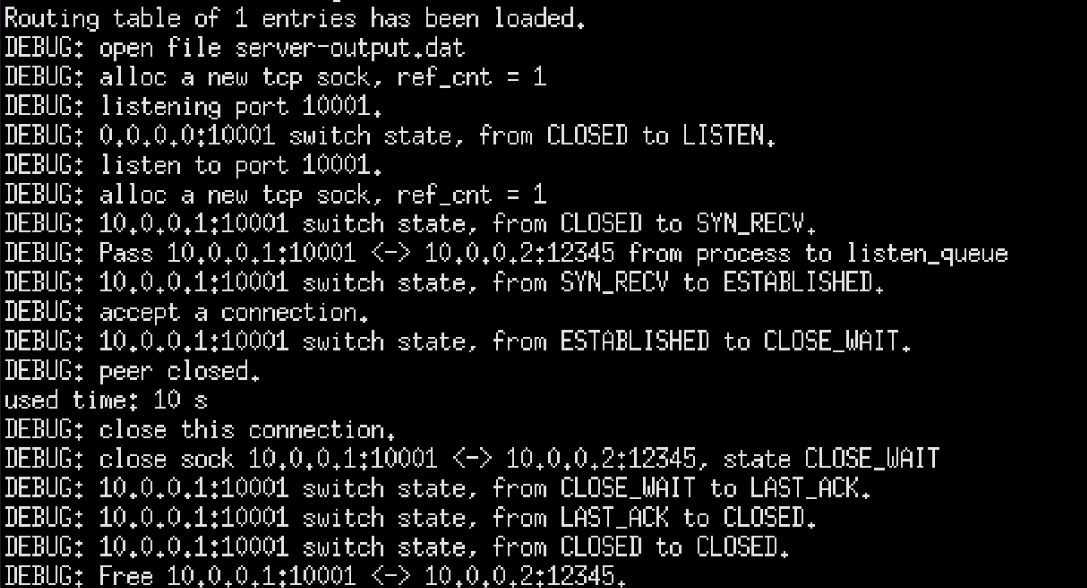
\includegraphics[width=0.7\textwidth]{my_server_my_client_h1.png}
        \caption{my\_server}
    \end{figure}

    \begin{figure}[H]
        \centering
        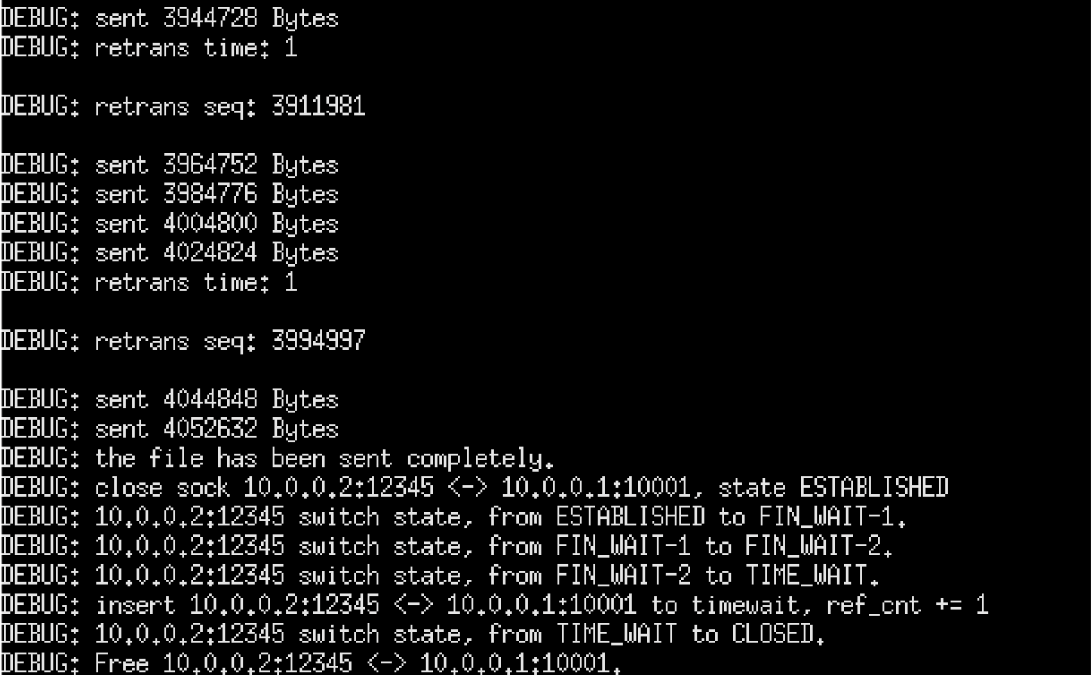
\includegraphics[width=0.7\textwidth]{my_server_my_client_h2.png}
        \caption{my\_client}
    \end{figure}

    \begin{figure}[H]
        \centering
        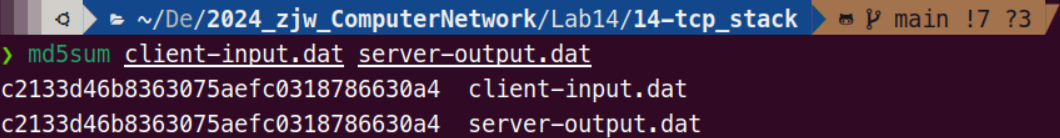
\includegraphics[width=0.7\textwidth]{my_server_my_client_md5sum.png}
        \caption{md5sum}
    \end{figure}

    可以看出,出现了丢包,但是通过重传机制,最终文件完全相同。

    \item 本实验server与标准client进行数据传输,用md5sum比较两个文件是否完全相同,结果如下:
    
    \begin{figure}[H]
        \centering
        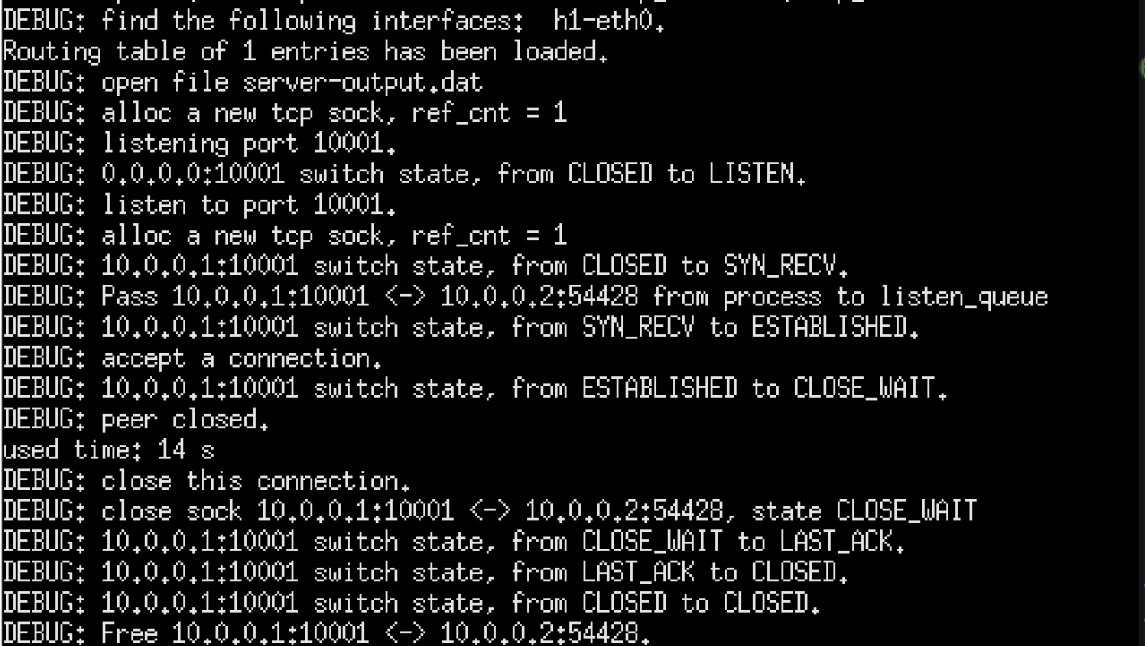
\includegraphics[width=0.7\textwidth]{my_server_std_client_h1.png}
        \caption{my\_server}
    \end{figure}

    \begin{figure}[H]
        \centering
        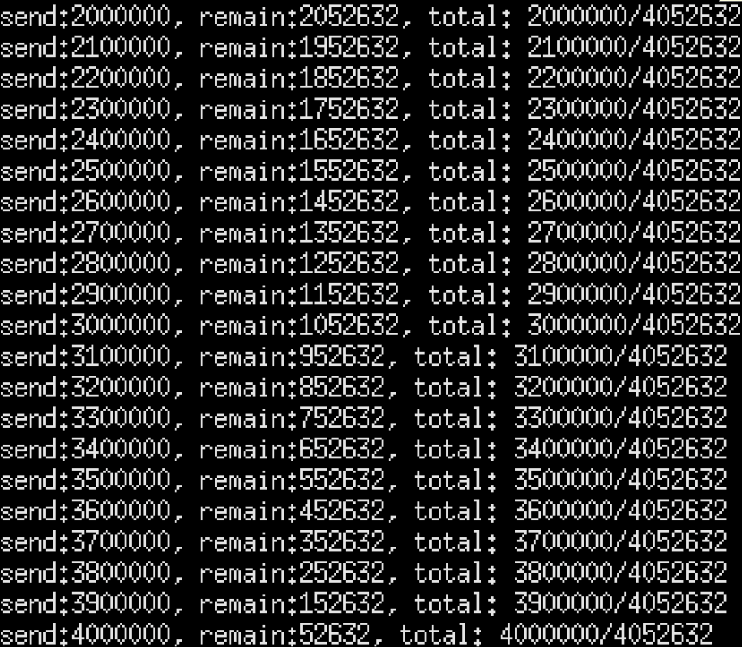
\includegraphics[width=0.7\textwidth]{my_server_std_client_h2.png}
        \caption{std\_client}
    \end{figure}

    \begin{figure}[H]
        \centering
        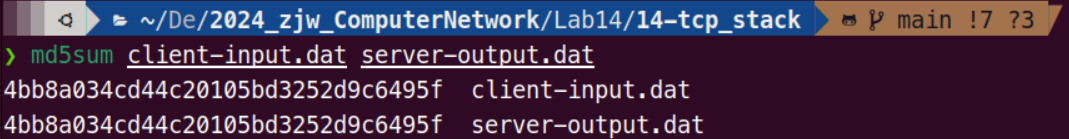
\includegraphics[width=0.7\textwidth]{my_server_std_client_md5sum.png}
        \caption{md5sum}
    \end{figure}

    可以看出,出现了丢包,但是通过重传机制,最终文件完全相同。

    \item 标准server与本实验client进行数据传输,用md5sum比较两个文件是否完全相同,结果如下:
    
    \begin{figure}[H]
        \centering
        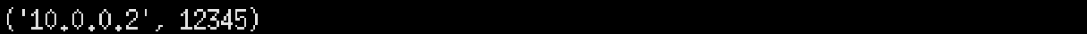
\includegraphics[width=0.7\textwidth]{std_server_my_client_h1.png}
        \caption{std\_server}
    \end{figure}

    \begin{figure}[H]
        \centering
        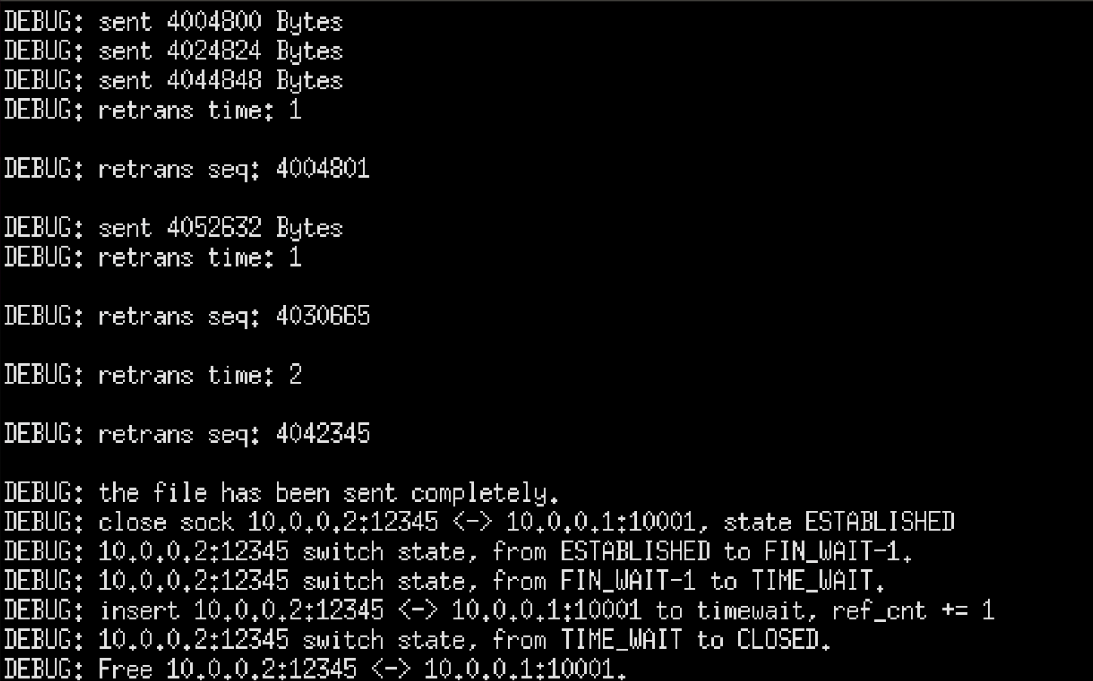
\includegraphics[width=0.7\textwidth]{std_server_my_client_h2.png}
        \caption{my\_client}
    \end{figure}

    \begin{figure}[H]
        \centering
        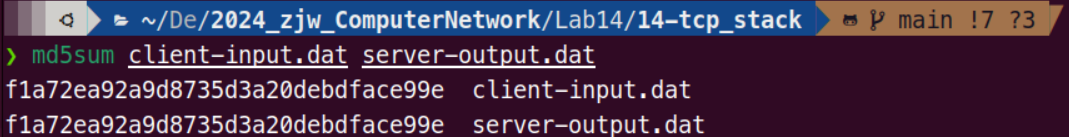
\includegraphics[width=0.7\textwidth]{std_server_my_client_md5sum.png}
        \caption{md5sum}
    \end{figure}

    可以看出,出现了丢包,但是通过重传机制,最终文件完全相同。
\end{enumerate}

\subsection{拥塞控制}

\section{实验总结}

本次实验中,我们实现了丢包恢复和拥塞控制的功能。通过实验,我们再次深入了解了 TCP 协议栈的工作原理。实现可靠传输使得数据传输更加稳定,实现拥塞控制使得网络更加稳定。通过本次实验,我们对 TCP 协议栈的实现有了更深入的了解,更加接近真实的 TCP 协议栈。


\end{document}